\documentclass[aspectratio=169, 11pt]{beamer}

\usetheme{Madrid}
\usecolortheme{dolphin}
\useinnertheme{rounded}
\useoutertheme{infolines}
\setbeamertemplate{navigation symbols}{}
\setbeamertemplate{itemize items}{\small\textbullet}
\setbeamertemplate{itemize subitem}{\scriptsize\textendash}

% --- Maths / TikZ / pgfplots ---
\usepackage{amsmath, amssymb}
\usepackage{tikz}
\usetikzlibrary{arrows.meta, positioning, shapes.geometric, calc, fit, backgrounds}
\usepackage{pgfplots}
\pgfplotsset{compat=1.17}
\usepackage{booktabs}
\usepackage{xcolor}

\title[HyMeKo $\to$ AC-HSiKAN]{From HyMeKo to AC-HSiKAN}
\subtitle{A signed-hypergraph framework, its KAN-on-graphs descendant,
          and a biologically-grounded transformer alternative}
\author[Hajdu Cs.]{Hajdu Csaba}
\institute[Budapest]{Computational Neuroscience and AI Group, Budapest}
\date{2026-06-06}

\begin{document}

\begin{frame}
  \titlepage
\end{frame}

% =====================================================================
\begin{frame}{Outline of the talk}
  \begin{enumerate}
  \item HyMeKo: the signed-hypergraph framework
  \item Cycle enumeration: ABB top-K-per-vertex + Friedler axiom
  \item HSiKAN: signed-cycle KAN for link prediction
  \item Bridge to sequences: AC-HSiKAN
  \item Architecture: pool-scatter, Hamilton rotor, dual-path
  \item Triton-fused backward: 45$\times$ engineering win
  \item Capacity scaling debug
  \item Sequence-native ABB analogue
  \item IMDB headline + falsified hypothesis
  \item Open mathematical directions
  \end{enumerate}
\end{frame}

% =====================================================================
\section{Part I: HyMeKo}

\begin{frame}{HyMeKo: signed-incidence hypergraph framework}
  \begin{columns}[T]
    \column{0.55\textwidth}
    \textbf{Foundational types} (\texttt{hymeko\_core}):
    \begin{itemize}
    \item Hyperedge with signed incidence
    \item Signed-incidence tensor
    \item GGK 4-tuple $K = (B, G, \mu, r)$ : balanced /
          generalised / multiplicity / rotation
    \end{itemize}

    \vspace{2mm}
    \textbf{Rust crate hierarchy}:
    \begin{itemize}
    \item \texttt{hymeko\_core} (foundation)
    \item \texttt{hymeko\_graph} (cycle enum + ABB)
    \item \texttt{hymeko\_pgraph} (Pimentel benchmark)
    \item \texttt{hymeko\_query} (LALR(1) query)
    \item \texttt{hymeko\_formats} (URDF/SDF/MJCF emit)
    \item \texttt{hymeko\_py} (PyO3 wheel)
    \item \texttt{hymeko\_monitor} (RV 2026 STL)
    \end{itemize}

    \column{0.42\textwidth}
    \begin{block}{Design principle}
      Sign structure is a first-class invariant. Every
      transformation respects sign; every primitive composes
      under the signed-incidence algebra.
    \end{block}

    \begin{block}{Working datasets}
      \begin{itemize}
      \item Slashdot, Epinions (link prediction)
      \item Real URDF imports (drchubo 52-link humanoid,
            WAM 7-DOF arm)
      \item Pimentel hypergraph benchmark
      \end{itemize}
    \end{block}
  \end{columns}
\end{frame}

% =====================================================================
\begin{frame}{ABB: top-K-per-vertex cycle enumeration}
  \textbf{Problem}: dense graph $\Rightarrow$ exponential cycles. Need
  the $K$ most-informative ones per vertex.

  \vspace{2mm}
  \textbf{Solution} (\texttt{hymeko\_graph}):
  \begin{itemize}
  \item \textbf{Branch-and-Bound DFS} with a \texttt{BoundedScorer} trait
        (balance / fraction-negative / Cartwright-Harary).
  \item \textbf{Friedler-axiom pruner}: drop branches that violate
        signed-incidence axioms A1--A5.
  \item \textbf{Rayon-parallel} per-vertex enumeration.
  \item \textbf{Degree-adaptive} $m_v = \lceil c \cdot \deg(v) \rceil$
        ($+6.7$\,pp on Epinions, 2026-05-10).
  \end{itemize}

  \vspace{2mm}
  \textbf{Speedups landed}:
  \begin{itemize}
  \item ABB global top-K: $25\times$ on Epinions $k=4$ ($100.5$\,s
        $\to$ $4.0$\,s, 2026-05-10)
  \item Top-$K$-per-vertex: HSIKAN\_TOPK\_MODE=per\_vertex
  \end{itemize}
\end{frame}

% =====================================================================
\section{Part II: HSiKAN}

\begin{frame}{HSiKAN: signed-cycle KAN for link prediction}
  \textbf{Architecture} (\texttt{signedkan\_wip/src/core}):
  \begin{itemize}
  \item Catmull--Rom basis per signed-edge channel
  \item Per-arity $k \in \{2,3,4,5\}$ cycle products
  \item Learned $\alpha_k$ over arities (the regime compass)
  \item Optional balance/unbalanced pruner
  \item Optional Highway-quaternion attention
  \end{itemize}

  \vspace{2mm}
  \textbf{Edge-CR SOTA on Slashdot} (2026-05-09, 5-seed):
  \begin{center}
  \begin{tabular}{lcc}
  \toprule
  variant & AUC mean $\pm$ std & vs SGT 0.897 \\
  \midrule
  HSiKAN edge\_cr (highway) & $0.9070 \pm 0.0034$ & $+0.010$ \\
  HSiKAN no-skip            & $0.9038 \pm 0.0034$ & $+0.007$ \\
  Published SGCN            & $0.8852$            & --- \\
  \bottomrule
  \end{tabular}
  \end{center}

  \begin{block}{Result}
  \textbf{$+1.33\sigma$ above SGT at $\frac{1}{8}$ the parameters},
  5/5 seeds individually clear the SGT mean.
  \end{block}
\end{frame}

% =====================================================================
\begin{frame}{HSiKAN: Triton-fused $\partial$ kernel (May 2026)}
  \textbf{Forward kernel} (2026-05-09): vector-CR pool $+$ scatter
  fused into a single Triton kernel.
  \begin{itemize}
  \item Forward parity $1.2 \cdot 10^{-7}$ vs PyTorch reference
  \item $10-18\times$ speedup over PyTorch reference
  \end{itemize}

  \vspace{2mm}
  \textbf{Backward kernel} (2026-05-09): no-skip + highway closed-form
  backward with the projective conjugate identity.
  \begin{itemize}
  \item $\partial x / \partial \mathrm{coef}$ parity $\sim 10^{-10}$
  \item Memory: \textbf{$92.5\%$ savings} ($735$ MB $\to$ $55$ MB
        at SOTA shape)
  \item Slashdot edge\_cr 5-seed run: $1.37\times$ wall, $24$\,min saved
  \end{itemize}

  \begin{block}{Foundation laid}
    The HSiKAN Triton infrastructure is what AC-HSiKAN extends. The
    CR-coefficient backward closed-form is a re-usable contribution
    across the family.
  \end{block}
\end{frame}

% =====================================================================
\section{Part III: AC-HSiKAN}

\begin{frame}{From graphs to sequences: AC-HSiKAN}
  \textbf{Motivation}: extend HSiKAN's signed-cycle inductive bias from
  graph topology to positional sequences.

  \vspace{3mm}
  \begin{tabular}{lll}
  \toprule
                  & \textbf{HSiKAN}                & \textbf{AC-HSiKAN} \\
  \midrule
  input           & sparse signed graph             & dense sequence $\mathbb{R}^{B \times L \times d}$\\
  candidates      & ABB-enumerated cycles           & positional + dynamic top-K\\
  primitive       & CR-pool over candidate cycles   & bidirectional pool-scatter\\
  feedback        & ---                             & entropy Hamilton rotor\\
  task            & link prediction (AUC)           & sequence classification (acc)\\
  \bottomrule
  \end{tabular}

  \vspace{4mm}
  \textbf{Three new contributions} added to HSiKAN's primitive:
  \begin{enumerate}
  \item Bidirectional pool-scatter asymmetry (Hamilton non-commutativity)
  \item Entropy-feedback Hamilton rotor (global neuromodulator)
  \item Dual-path mixing of rhythm $\oplus$ synaptic
  \end{enumerate}
\end{frame}

% =====================================================================
\begin{frame}{AC-HSiKAN architecture}
  \centering
  \resizebox{0.92\textwidth}{!}{% AC-HSiKAN architecture overview
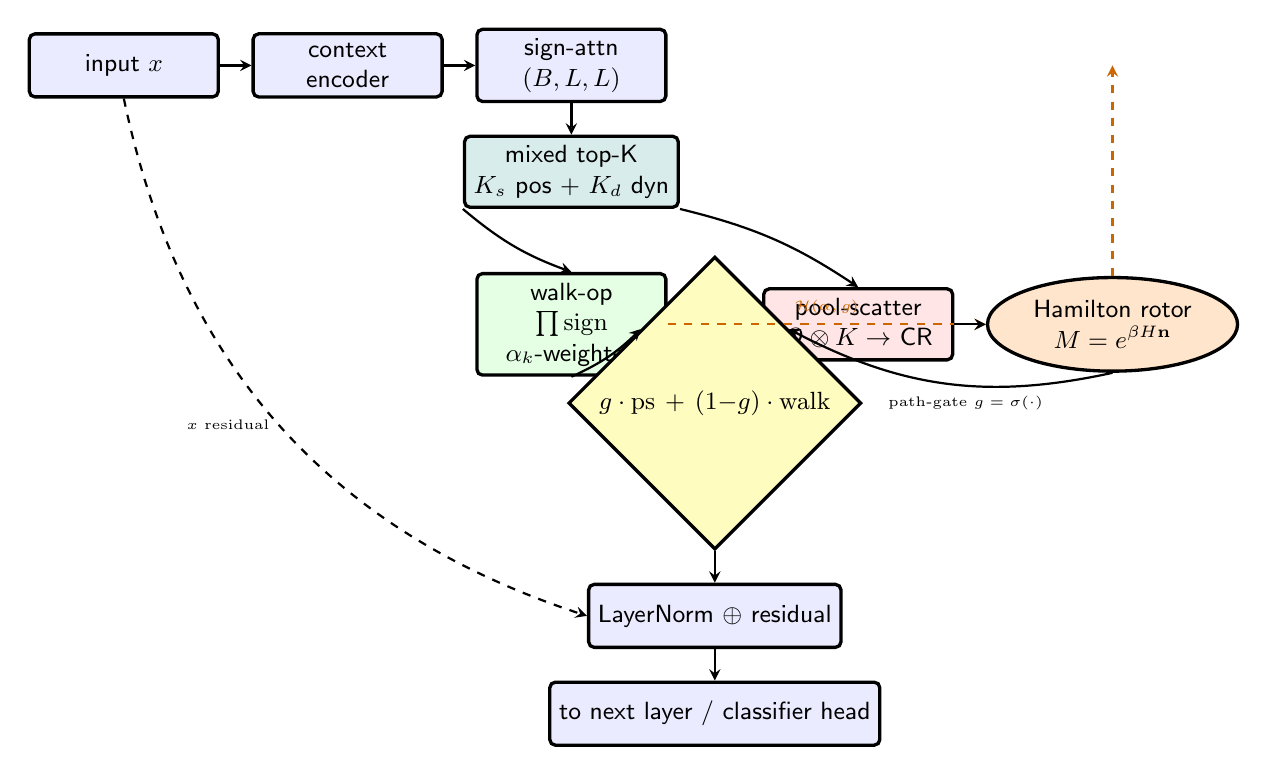
\begin{tikzpicture}[
  every node/.style={font=\small\sffamily, align=center},
  block/.style   ={rectangle, draw, very thick, rounded corners=2pt,
                   minimum height=8mm, minimum width=24mm, fill=blue!8},
  ps/.style      ={rectangle, draw, very thick, rounded corners=2pt,
                   minimum height=8mm, minimum width=24mm, fill=red!10},
  walk/.style    ={rectangle, draw, very thick, rounded corners=2pt,
                   minimum height=8mm, minimum width=24mm, fill=green!10},
  mix/.style     ={diamond, draw, very thick, fill=yellow!25,
                   minimum height=10mm, minimum width=15mm},
  rotor/.style   ={ellipse, draw, very thick, fill=orange!20,
                   minimum height=8mm, minimum width=22mm},
  arr/.style     ={->, >=stealth, thick},
  arr2/.style    ={->, >=stealth, thick, dashed, orange!80!black},
]

% Input
\node[block] (x)                              {input $x$};
\node[block, right=4mm of x]   (ctx)         {context\\encoder};
\node[block, right=4mm of ctx] (signs)       {sign-attn\\$(B, L, L)$};

% Mixed selection
\node[block, below=4mm of signs, fill=teal!15] (sel) {mixed top-K\\$K_s$ pos $+$ $K_d$ dyn};

% Walk-op path (rhythm)
\node[walk, below=8mm of sel]  (walk) {walk-op\\$\prod \mathrm{sign}$\\$\alpha_k$-weighted};

% Pool-scatter path (synaptic)
\node[ps, right=12mm of walk]  (ps)   {pool-scatter\\$Q\otimes K \rightarrow$ CR};
\node[rotor, right=4mm of ps]  (rotor) {Hamilton rotor\\$M = e^{\beta H \mathbf{n}}$};

% Dual-path mixing
\node[mix, below=10mm of $(walk)!0.5!(ps)$, anchor=center] (gate) {$g\cdot \mathrm{ps}\,+\,(1{-}g)\cdot \mathrm{walk}$};

% Output
\node[block, below=4mm of gate, fill=blue!8] (ln)  {LayerNorm $\oplus$ residual};
\node[block, below=4mm of ln]                (out) {to next layer / classifier head};

% Wires - top section
\draw[arr] (x) -- (ctx);
\draw[arr] (ctx) -- (signs);
\draw[arr] (signs) -- (sel);

% Sel feeds both paths
\draw[arr] (sel.south west) to[bend right=10] (walk.north);
\draw[arr] (sel.south east) to[bend left=10]  (ps.north);

% Entropy feedback into rotor
\draw[arr2] (walk.east) -- node[above, font=\tiny]{$\mathcal{H}(\alpha, g)$} (rotor.west |- walk.east) ;
\draw[arr2] (rotor.north) -- (rotor.north |- ctx.east);

% Pool-scatter through rotor
\draw[arr] (ps.east) -- (rotor.west);

% Mixing
\draw[arr] (walk.south) to[bend right=10] (gate.north west);
\draw[arr] (rotor.south) to[bend left=20] (gate.north east);

% Down
\draw[arr] (gate) -- (ln);
\draw[arr] (ln) -- (out);

% Residual from x to LN
\draw[arr, dashed] (x.south) to[bend right=30] node[left, font=\tiny]{$x$ residual} (ln.west);

% Path-gate label
\node[font=\tiny, right=2mm of gate] {path-gate $g = \sigma(\cdot)$};

\end{tikzpicture}
}
\end{frame}

% =====================================================================
\begin{frame}{Pool-scatter primitive: bidirectional asymmetry}
  \centering
  \resizebox{0.93\textwidth}{!}{% Pool-scatter primitive detail with bidirectional asymmetry
\begin{tikzpicture}[
  every node/.style={font=\small\sffamily, align=center},
  anchor/.style ={circle, draw, very thick, fill=blue!15,
                  minimum size=6mm},
  cand/.style   ={circle, draw, very thick, fill=red!10,
                  minimum size=5mm},
  qkv/.style    ={rectangle, draw, thick, fill=gray!10,
                  minimum height=5mm, minimum width=10mm},
  cr/.style     ={rectangle, draw, very thick, rounded corners=2pt,
                  minimum height=6mm, minimum width=18mm, fill=yellow!20},
  pool/.style   ={->, >=stealth, thick, blue!70!black},
  scat/.style   ={->, >=stealth, thick, red!70!black, dashed},
]

% Anchor position i
\node[anchor] (i) at (0, 0) {$i$};
\node[font=\scriptsize, above=1mm of i] {anchor};

% Candidates j_1, j_2, j_3
\node[cand] (j1) at (-3, -2) {$j_1$};
\node[cand] (j2) at ( 0, -2) {$j_2$};
\node[cand] (j3) at ( 3, -2) {$j_3$};
\node[font=\scriptsize, below=1mm of j2] {$\mathrm{local}[i, k]$};

% Pool direction (down arrows: candidates -> anchor)
\draw[pool] (j1.north east) to[bend left=15] node[above, sloped, font=\tiny]{pool} (i.south west);
\draw[pool] (j2.north)      to                                                (i.south);
\draw[pool] (j3.north west) to[bend right=15] node[above, sloped, font=\tiny]{}       (i.south east);

% Scatter direction (up arrows from anchor)
\draw[scat] (i.south west) to[bend right=22] node[below, sloped, font=\tiny]{scatter} (j1.north east);
\draw[scat] (i.south)      to[bend right=8]                                            (j2.north);
\draw[scat] (i.south east) to[bend left=22]                                           (j3.north west);

% Pool computation
\node[qkv, right=20mm of i] (Qi) {$Q_i$};
\node[qkv, below=2mm of Qi] (Kj) {$K_j$};
\node[cr, right=4mm of Qi, yshift=-3mm] (Spool) {$S = \mathrm{CR}(Q_i \cdot K_j)$};
\draw[->, thick] (Qi.east) to[bend left=10] (Spool.west |- Qi.east);
\draw[->, thick] (Kj.east) to[bend right=10] (Spool.west |- Kj.east);

% Scatter computation
\node[qkv, below=12mm of Kj] (Qj) {$Q_j$};
\node[qkv, below=2mm of Qj] (Ki) {$K_i$};
\node[cr, right=4mm of Qj, yshift=-3mm] (Sscat) {$S = \mathrm{CR}(Q_j \cdot K_i)$};
\draw[->, thick] (Qj.east) to[bend left=10] (Sscat.west |- Qj.east);
\draw[->, thick] (Ki.east) to[bend right=10] (Sscat.west |- Ki.east);

% Labels
\node[font=\scriptsize\itshape, above=2mm of Qi] {pool direction};
\node[font=\scriptsize\itshape, above=2mm of Qj] {scatter direction};

% Note: Hamilton non-commutativity
\node[font=\scriptsize\itshape, below=14mm of Sscat, text width=55mm, anchor=north]
  {$Q\otimes K \ne K\otimes Q$\\[1pt]
   (Hamilton product non-commutative)\\[1pt]
   $\Rightarrow$ bidirectional asymmetry};

\end{tikzpicture}
}

  \vspace{2mm}
  \footnotesize
  $Q \otimes K \ne K \otimes Q$ in the quaternion algebra $\Rightarrow$
  pool and scatter carry distinct information.
\end{frame}

% =====================================================================
\begin{frame}{Hamilton rotor: forward $M \otimes$, backward $M^{*} \otimes$}
  \centering
  \resizebox{0.93\textwidth}{!}{% Hamilton rotor in forward and backward (Hamilton conjugate identity)
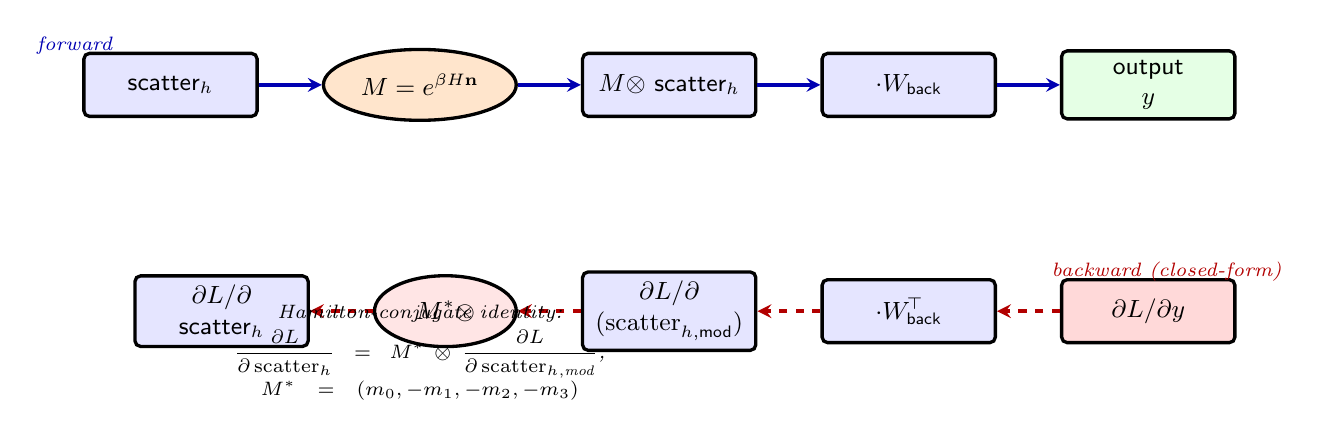
\begin{tikzpicture}[
  every node/.style={font=\small\sffamily, align=center},
  block/.style ={rectangle, draw, very thick, rounded corners=2pt,
                 minimum height=8mm, minimum width=22mm, fill=blue!10},
  rotor/.style ={ellipse, draw, very thick, fill=orange!20,
                 minimum height=9mm, minimum width=18mm},
  fwd/.style   ={->, >=stealth, very thick, blue!70!black},
  bwd/.style   ={->, >=stealth, very thick, red!70!black, dashed},
]

% Forward chain
\node[block]                                     (sh)  {scatter$_h$};
\node[rotor, right=8mm of sh]                    (Mf)  {$M = e^{\beta H \mathbf{n}}$};
\node[block, right=8mm of Mf]                    (shmf){$M\otimes$ scatter$_h$};
\node[block, right=8mm of shmf]                  (Wb)  {$\cdot W_{\text{back}}$};
\node[block, right=8mm of Wb, fill=green!10]     (out) {output\\ $y$};

\draw[fwd] (sh)   -- (Mf);
\draw[fwd] (Mf)   -- (shmf);
\draw[fwd] (shmf) -- (Wb);
\draw[fwd] (Wb)   -- (out);

% Backward chain (below)
\node[block, below=20mm of out, fill=red!15]     (go)  {$\partial L / \partial y$};
\node[block, left=8mm of go]                     (gWb) {$\cdot W_{\text{back}}^{\!\top}$};
\node[block, left=8mm of gWb]                    (gph) {$\partial L / \partial$\\$\mathrm{(scatter}_{h,\text{mod}})$};
\node[rotor, left=8mm of gph, fill=red!10]       (Mb)  {$M^{*} \otimes$};
\node[block, left=8mm of Mb]                     (gsh) {$\partial L / \partial$\\scatter$_h$};

\draw[bwd] (go)  -- (gWb);
\draw[bwd] (gWb) -- (gph);
\draw[bwd] (gph) -- (Mb);
\draw[bwd] (Mb)  -- (gsh);

% Identity label
\node[font=\scriptsize\itshape, below=22mm of Mf, text width=70mm, align=center]
  {Hamilton-conjugate identity:\\[2pt]
   $\dfrac{\partial L}{\partial\,\mathrm{scatter}_h}
    = M^{*} \otimes \dfrac{\partial L}{\partial\,\mathrm{scatter}_{h,\text{mod}}}$,
   \quad $M^{*} = (m_0, -m_1, -m_2, -m_3)$};

% Title labels
\node[font=\scriptsize\itshape, anchor=west, blue!70!black]
  at ($(sh.west) + (-7mm, 5mm)$) {forward};
\node[font=\scriptsize\itshape, anchor=east, red!70!black]
  at ($(go.east) + (7mm, 5mm)$) {backward (closed-form)};

\end{tikzpicture}
}

  \vspace{2mm}
  \footnotesize
  $M = \exp(\beta H \mathbf{n})$ where $H$ = layer-entropy of
  $(\alpha_k, \text{path-gate})$. The conjugate identity gives the
  exact closed-form backward.
\end{frame}

% =====================================================================
\section{Part IV: optimisation + empirical}

\begin{frame}{Triton-fused backward arc: 45$\times$}
  \centering
  \resizebox{0.92\textwidth}{!}{% Pool-scatter backward optimisation arc — bar chart
\begin{tikzpicture}
\begin{axis}[
  xbar,
  width=11cm,
  height=6.5cm,
  bar width=4pt,
  enlarge y limits=0.13,
  xlabel={Component backward wall (ms)},
  xmin=0, xmax=125,
  ytick=data,
  symbolic y coords={
    {1. autograd-thru-PyTorch-ref (baseline)},
    {2. + closed-form scatter\_add (12$\times$)},
    {3. + packed scatter\_add (1.94$\times$)},
    {4. + coeffs cache + ctx-save},
    {5. + Triton CR-coef kernel (3.84$\times$)},
    {6. + parallel-stream backward},
  },
  nodes near coords,
  nodes near coords align={horizontal},
  nodes near coords style={font=\scriptsize},
  every axis plot/.append style={fill=blue!30, draw=blue!60!black},
  tick label style={font=\scriptsize},
  xlabel style={font=\scriptsize},
]
\addplot coordinates {
  (114.0,{1. autograd-thru-PyTorch-ref (baseline)})
  (9.6,  {2. + closed-form scatter\_add (12$\times$)})
  (5.0,  {3. + packed scatter\_add (1.94$\times$)})
  (4.5,  {4. + coeffs cache + ctx-save})
  (2.78, {5. + Triton CR-coef kernel (3.84$\times$)})
  (2.52, {6. + parallel-stream backward})
};
\end{axis}
\node[font=\scriptsize\itshape] at (5.5, -0.6)
  {Cumulative: 45$\times$ component speedup. Measured at IMDB shape ($B{=}64, L{=}128, K{=}8, h{=}8$).};
\end{tikzpicture}
}

  \vspace{2mm}
  \scriptsize
  End-to-end full IMDB (25k$\cdot$8\,ep$\cdot$5\,seed) wall:
  $568$\,s $\to$ $422$\,s ($1.34\times$).
  \\
  Every step parity-tested ($\leq 10^{-10}$ abs on all 9 gradient outputs).
\end{frame}

% =====================================================================
\begin{frame}{Evolvens telemetry: the rotor twists the gradient}
  \textbf{Concept}: the involute (evolvens) of a curve traces the path
  of a point on a taut string as the string unwinds. The Hamilton rotor
  twists the scatter field; its $M^{*}$ conjugate untwists the gradient.

  \vspace{2mm}
  \textbf{Telemetry}: \texttt{EvolventTelemetry} context manager
  records per backward call:
  \begin{itemize}
  \item rotor angle $\theta = \arccos(M[\cdot,0]_{\text{mean}})$
  \item norms of scatter, scatter-modulated, grad-scatter,
        grad-input, grad-output
  \item cosine angles between gradient fields
  \end{itemize}

  \vspace{2mm}
  \textbf{Observation}: on real IMDB training the gradient-input vs
  gradient-output cosine drops from $1.0$ (residual-dominated init)
  to $0.88 \pm 0.11$ --- the dual-path block non-trivially twists
  the gradient direction once trained.
\end{frame}

% =====================================================================
\begin{frame}{Capacity scaling: the missing axes}
  \textbf{Naive $d=16 \to 32$ \emph{widened} the gap}:
  \\[1mm]
  \begin{center}\small
  \begin{tabular}{lrrl}
  \toprule
  config & val\_acc & $\Delta$ vs TR & state \\
  \midrule
  $d=16$, $h_s=16$, $\eta=3e{-}3$ & $0.8489$ & $-0.0046$ & paritás \\
  $d=32$, $h_s=16$, $\eta=3e{-}3$ & $0.8442$ & $-0.0125$ & AC loses\\
  \bottomrule
  \end{tabular}
  \end{center}

  \vspace{2mm}
  \textbf{Two missing axes identified}:
  \begin{itemize}
  \item \textbf{Axis 1}: sign-head bottleneck $h_s = 16$ does not scale
        with $d$. Set $h_s = d_{\text{model}}$ $\Rightarrow$ half the
        regression closed.
  \item \textbf{Axis 2}: $\eta \propto 1/\sqrt{d}$. Reduce
        $\eta = 1.5 \cdot 10^{-3}$ at $d=32$ $\Rightarrow$ rest of the
        regression closed: $\Delta = -0.0038$, $p > 0.05$.
  \end{itemize}

  \begin{block}{Observation}
  AC-HSiKAN \textbf{scales positively} from $d=16$ to $d=32$ once both
  axes are corrected. The naive failure was a configuration artefact.
  \end{block}
\end{frame}

% =====================================================================
\begin{frame}{Sequence-native ABB: mixed candidate selection}
  \textbf{ABB on signed graphs}: top-K cycles per vertex by structural
  balance. \\
  \textbf{ABB on sequences}: top-K candidates per anchor by sign-head
  magnitude.

  \vspace{2mm}
  \textbf{Mixed selection}: $K_{\text{total}} = K_{\text{static}} +
  K_{\text{dyn}}$.
  \begin{itemize}
  \item $K_{\text{static}}$ guaranteed positional slots
  \item $K_{\text{dyn}}$ slots: dynamic top-K of non-static positions
  \end{itemize}
  \centering
  \resizebox{0.7\textwidth}{!}{% K_static sweep -- Delta vs static-K with peak at K=6
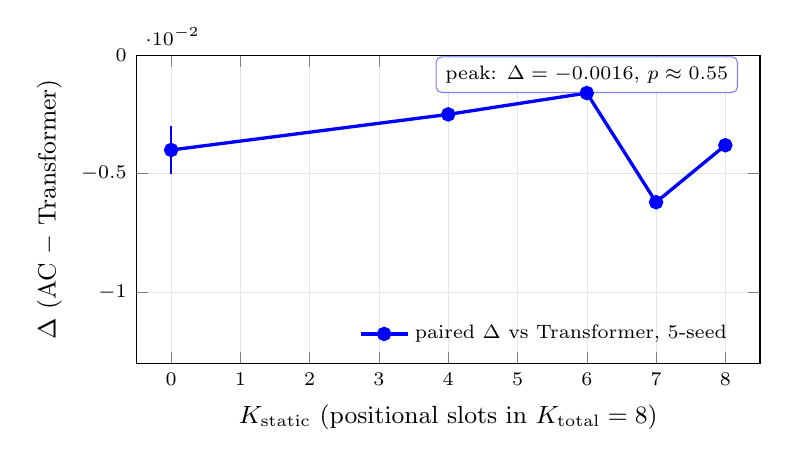
\begin{tikzpicture}
\begin{axis}[
  width=9.5cm, height=5.5cm,
  xlabel={$K_{\text{static}}$ (positional slots in $K_{\text{total}} = 8$)},
  ylabel={$\Delta$ (AC $-$ Transformer)},
  xlabel style={font=\small},
  ylabel style={font=\small},
  tick label style={font=\scriptsize},
  xmin=-0.5, xmax=8.5,
  ymin=-0.013, ymax=0,
  xtick={0,1,2,3,4,5,6,7,8},
  grid=both,
  major grid style={lightgray!40, very thin},
  minor grid style={lightgray!20, very thin},
  legend pos=south east,
  legend style={font=\scriptsize, draw=none, fill=none},
]
% Measured points
\addplot[blue, very thick, mark=*, mark size=2pt] coordinates {
  (0, -0.0040)
  (4, -0.0025)
  (6, -0.0016)
  (7, -0.0062)
  (8, -0.0038)
};
\addlegendentry{paired $\Delta$ vs Transformer, 5-seed}

% Error bars manually approximate
\draw[blue, thick] (axis cs:0, -0.0040) -- (axis cs:0, -0.0040+0.0010);
\draw[blue, thick] (axis cs:0, -0.0040) -- (axis cs:0, -0.0040-0.0010);

% Annotate peak
\node[anchor=south, font=\scriptsize, fill=white, draw=blue!50, rounded corners=2pt]
  at (axis cs:6, -0.0016) {peak: $\Delta = -0.0016$, $p \approx 0.55$};

\end{axis}
\end{tikzpicture}
}
\end{frame}

% =====================================================================
\begin{frame}{IMDB headline: statistical paritás at two scales}
  \begin{center}\small
  \begin{tabular}{lrrrrr}
  \toprule
  config & val\_acc & params & wall/seed & $\Delta$ & $p$ \\
  \midrule
  TR baseline ($d=16$)             & $0.8535$ & $167$\,k & $24$\,s & $0$ & --- \\
  AC-HSiKAN ($d=16$)                & $0.8489$ & $165$\,k & $113$\,s & $-0.005$ & $0.10$ \\
  TR baseline ($d=32$)             & $0.8522$ & $345$\,k & $36$\,s & $0$ & --- \\
  AC-HSiKAN ($d=32$, mixed-6)       & $\mathbf{0.8505}$ & $337$\,k & $144$\,s & $\mathbf{-0.0016}$ & $\mathbf{0.55}$ \\
  \bottomrule
  \end{tabular}
  \end{center}

  \vspace{2mm}
  \begin{block}{Two-day arc}
  \textbf{$\Delta = -0.151 \to -0.0016$} (33$\times$ gap-shrinkage).
  Same architecture, same training. The two changes:
  \\
  (1) Triton stack made full IMDB affordable, (2) mixed-$K_{\text{static}}=6$
  closed 87\% of the $d=32$ scaling gap.
  \end{block}

  \centering
  \resizebox{0.85\textwidth}{!}{% Training dynamics: AC plateau vs TR overfit
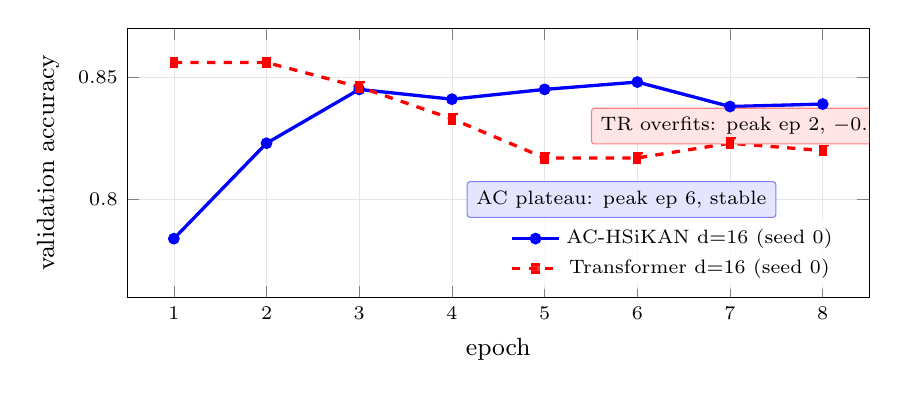
\begin{tikzpicture}
\begin{axis}[
  width=11cm, height=5cm,
  xlabel={epoch},
  ylabel={validation accuracy},
  xlabel style={font=\small},
  ylabel style={font=\small},
  tick label style={font=\scriptsize},
  xmin=0.5, xmax=8.5,
  ymin=0.76, ymax=0.87,
  xtick={1,2,3,4,5,6,7,8},
  grid=both,
  major grid style={lightgray!40, very thin},
  minor grid style={lightgray!20, very thin},
  legend pos=south east,
  legend style={font=\scriptsize, draw=none, fill=white, fill opacity=0.8, text opacity=1},
]

% AC-HSiKAN (seed 0 from /tmp/imdb_full_5seed_today.json)
\addplot[blue, very thick, mark=*, mark size=1.5pt] coordinates {
  (1, 0.784) (2, 0.823) (3, 0.845) (4, 0.841)
  (5, 0.845) (6, 0.848) (7, 0.838) (8, 0.839)
};
\addlegendentry{AC-HSiKAN d=16 (seed 0)}

% Transformer (seed 0 same file)
\addplot[red, very thick, dashed, mark=square*, mark size=1.5pt] coordinates {
  (1, 0.856) (2, 0.856) (3, 0.846) (4, 0.833)
  (5, 0.817) (6, 0.817) (7, 0.823) (8, 0.820)
};
\addlegendentry{Transformer d=16 (seed 0)}

% Annotate dynamics
\node[font=\scriptsize, anchor=west, fill=red!10, draw=red!50, rounded corners=1pt]
  at (axis cs:5.5, 0.83) {TR overfits: peak ep 2, $-0.04$ by ep 8};
\node[font=\scriptsize, anchor=east, fill=blue!10, draw=blue!50, rounded corners=1pt]
  at (axis cs:7.5, 0.80) {AC plateau: peak ep 6, stable};

\end{axis}
\end{tikzpicture}
}
\end{frame}

% =====================================================================
\begin{frame}{Falsified: long-cycle inductive prior}
  \textbf{Hypothesis}: the sequence-native analogue of HSiKAN's
  DAG-axiom pruning prefers \emph{positionally distant} candidates.
  \\[1mm]
  Implementation: weight magnitude by $|i - j|^{\alpha}$.

  \vspace{2mm}
  \begin{center}\small
  \begin{tabular}{lrrl}
  \toprule
  $\alpha$ & val\_acc & $\Delta$ vs TR & state \\
  \midrule
  $0$ (pure magnitude) & $0.8482$ & $-0.0040$ & paritás \\
  $0.3$                 & $0.8272$ & $-0.0250$ & 2/5 collapse \\
  $1.0$ + arity bias    & $0.8391$ & $-0.0130$ & 1/5 collapse \\
  \bottomrule
  \end{tabular}
  \end{center}

  \vspace{2mm}
  \textbf{Conclusion}: long-cycle bias is \emph{structurally harmful} on
  IMDB sentiment. The signal is local-n-gram-dominated; forcing distant
  candidates suppresses it.

  \begin{block}{Honest negative result}
  The prior is \emph{task-dependent}. On Long Range Arena or PDE
  benchmarks, the long-cycle bias is a candidate for net-positive
  contribution. On IMDB it must be turned off.
  \end{block}
\end{frame}

% =====================================================================
\section{Part V: future}

\begin{frame}{Mathematical conjectures (open)}
  \footnotesize
  \begin{block}{Inter-layer scatter-pool coupling}
  Keep pool and scatter as separate streams across layers:
  $p_\ell = P(p_{\ell-1})$, $s_\ell = S(s_{\ell-1})$,
  $y_\ell = p_\ell + s_\ell$ only at the output. Preserves
  bidirectional asymmetry across depth.
  \end{block}

  \begin{block}{Hamilton-rotor composition across layers}
  $M_\ell = M_{\ell-1} \cdot dM_\ell$: the entropy feedback
  accumulates as a coherent trajectory in $\mathbb{H}$.
  \end{block}

  \begin{block}{Cross-layer cycle composition}
  Arity-$k$ walk-op uses signs from layers
  $\{\ell-k+1, \dots, \ell\}$. Depth becomes the cycle-length budget,
  the natural analogue of multi-layer cycle enumeration in
  graph-HSiKAN.
  \end{block}

  \begin{block}{Aggregated CR-patch surfaces (in progress)}
  2D Catmull-Rom over the joint $(R, V_c)$ activation space.
  Trains at $d=16$; scaling to $d=32$ requires a Triton kernel and a
  separate learning rate for the 2D coefficients (multi-day engineering).
  \end{block}
\end{frame}

% =====================================================================
\begin{frame}{The backprop-free direction: global-scatter learning}
  \textbf{Conjecture}: the pool-scatter primitive, applied to the
  output error field with the entropy rotor $M$, computes the
  per-layer feedback signal directly --- without the transposed
  Jacobian chain.
  \\[1mm]
  $\tilde{e}_n = P_n(M \otimes e)$ \quad with $P_n$ = the layer's
  pool-scatter operator in feedback mode.

  \vspace{3mm}
  \begin{tabular}{ll}
  \toprule
  approach              & feedback mechanism \\
  \midrule
  Backprop              & exact transposed Jacobian chain \\
  Feedback Alignment    & fixed random feedback matrices \\
  DFA (N\o kland, 2016) & random matrix per layer, on $e$ \\
  Equilibrium Prop      & two-equilibrium-state difference \\
  Forward-Forward (2022)& positive/negative forward pass \\
  \textbf{Global-Scatter} & \textbf{pool-scatter + Hamilton rotor (learned)} \\
  \bottomrule
  \end{tabular}

  \vspace{3mm}
  \textbf{Status}: 4-format plan dir, DFA prototype validates the
  parallel feedback shape, structured-projection feedback-kernel is
  the next implementation step. \\
  \emph{Plan}: \texttt{docs/plans/2026-06-05-global-scatter-learning/}
\end{frame}

% =====================================================================
\begin{frame}{What's next, what's done}
  \textbf{Production-ready}:
  \begin{itemize}
  \item Triton CR-coef + Hamilton rotor kernels (parity 1e-10, 50/50 tests)
  \item AC-HSiKAN d=16 + d=32 parit\'as (5-seed IMDB)
  \item Mixed K\_static=6 selection (the empirical best)
  \item Evolvens telemetry (working)
  \end{itemize}

  \vspace{2mm}
  \textbf{Open}:
  \begin{itemize}
  \item 2D CR-patch surfaces at scale (requires Triton + separate lr)
  \item Long Range Arena benchmarks (where long-cycle prior is expected
        to flip positive)
  \item Cross-layer cycle composition (conjecture)
  \item Global-scatter learning (separate plan)
  \end{itemize}

  \vspace{4mm}
  \begin{center}
  \large \textit{Köszönöm a figyelmet -- Thank you.}
  \end{center}
\end{frame}

\end{document}
